\section{Results}
\label{sec:results}

% this section must be devoid of opinion

% Q1: is the solution off-chain?
% M1: number of changes to the blockchain protocol

The first question we asked was whether the solution was off-chain.
Our metric was the number of changes to the blockchain protocol. 
Our solution runs independently of a blockchain, making zero changes to the actual protocol.
However, it does ask that blockchain members participate in a new system, in addition to the blockchain. 

% Q2: is the solution efficient?
% M2: asymptotic analysis of time and space requirements as the chain grows
% M3: bytes of network traffic generated

We also wanted to know whether the solution is efficient.
We presented two metrics: asymptotic time and space analysis and the amount of network traffic generated.
Recording and analyzing network data turned out to be to too ambitious and is left for future work.
We do have the asymptotic analysis.
Suppose that a blockchain contains $n$ blocks and we consider an election between miners of the last $k$ blocks.
Regular blockchain protocol requires $O(n)$ processing time and space to bootstrap.
In our protocol, the space requirements actually has nothing to do with $n$ the total number of blocks.
Instead, each voter casts 2 votes.
Since there are $k$ voters our space is $O(k)$ linear in $k$.
Now for time analysis.
All the algorithms involved in the protocol take linear time in the number of votes so the run time for the protocol is also $O(k)$.

\begin{center}
\begin{table}[h]
    \centering
    \begin{tabular}{|l|l|l|l|}
        \hline
                  & Max time & Min time & Average time \\ \hline
        Algorand  & 2149 s   & 758 s    & 939  s       \\ \hline
        Bitcoin   & 1512 s   & 796 s    & 1038 s       \\ \hline
        Ethereum  & 2243 s   & 711 s    & 1108 s       \\ \hline
    \end{tabular}
    \caption{INSERT CAPTION}
    \label{tab:gqm}
\end{table}
\end{center}


Table \ref{tab:times} provides simulation time information extracted from our experiments.
For our experiments, we used the key distribution from three different blockchains: Algorand, Bitcoin, and Ethereum.
On average, the simulation ran for about 1000 seconds.
It should be noted that the simulation time is merely a lower bound for how long the protocol runs.
In real life, this depends on how quickly votes are cast.
We did not model delay in the voting protocol, meaning we are left with a lower bound.

% Q3: is the solution secure?
% M4: theoretical probability that a malicious actor fools a bootstrapping node
% M5: empirical probability that a malicious actor fools a bootstrapping node

The final question we wanted to explore asked how secure our system is.
Our metrics involve the probability (theoretical and empirical) that a malicious actor is able to fool a bootstrapping node into accepting a dishonest state.
Since the statistics remains up in the air, this question cannot be answered in its entirety.
However, we can report how much voting power an attacker can gain using different strategies.
Recall that the election is decided based on the vote distribution, so if an attacker is able to make a proportional gain, they gain an advantage in the election.
This means proportional gain is closely related to the probability that the attacker can fool a bootstrapping node.

We explore two strategies; the first is a deleting strategy.
In this attack, a naive dishonest manager wants to gain power in the election by deleting honest votes, increasing the attacker's voting power.
The goal of our protocol was to make it so that deleting votes left the ratio largely unchanged.
To simulate this attack, we produced an election and randomly selected one manager to be dishonest.
This manager then deleted each vote (one at a time) to see whether the election could be affected.
Figure \ref{fig:deleter} shows the gain for the three key distributions Algorand, Bitcoin, and Ethereum. 
We chose to order the votes along the $x$-axis by the round it was submitted in.
This shows how deleting a vote has different a affect depending on when it was submitted.
For Algorand and Bitcoin, the proportional gain drops below $5\%$ by round 8.
Ethereum also remains below $5\%$ gain beyond round 8 but we also have an added artifact that the attacker can continue to lose  up to 20\% of voting power through round 18.
The number of remaining valid votes, after deleting a vote, follows the same trend in each of the three key distributions.
As the vote's round increases, so does the number of votes that remain valid.
By round 8, there remain about 400 valid votes after a vote is deleted.
The number of remaining valid votes can be used to determine the minimum votes threshold in the decision mechanism.

\begin{figure}[h]
	\centering
	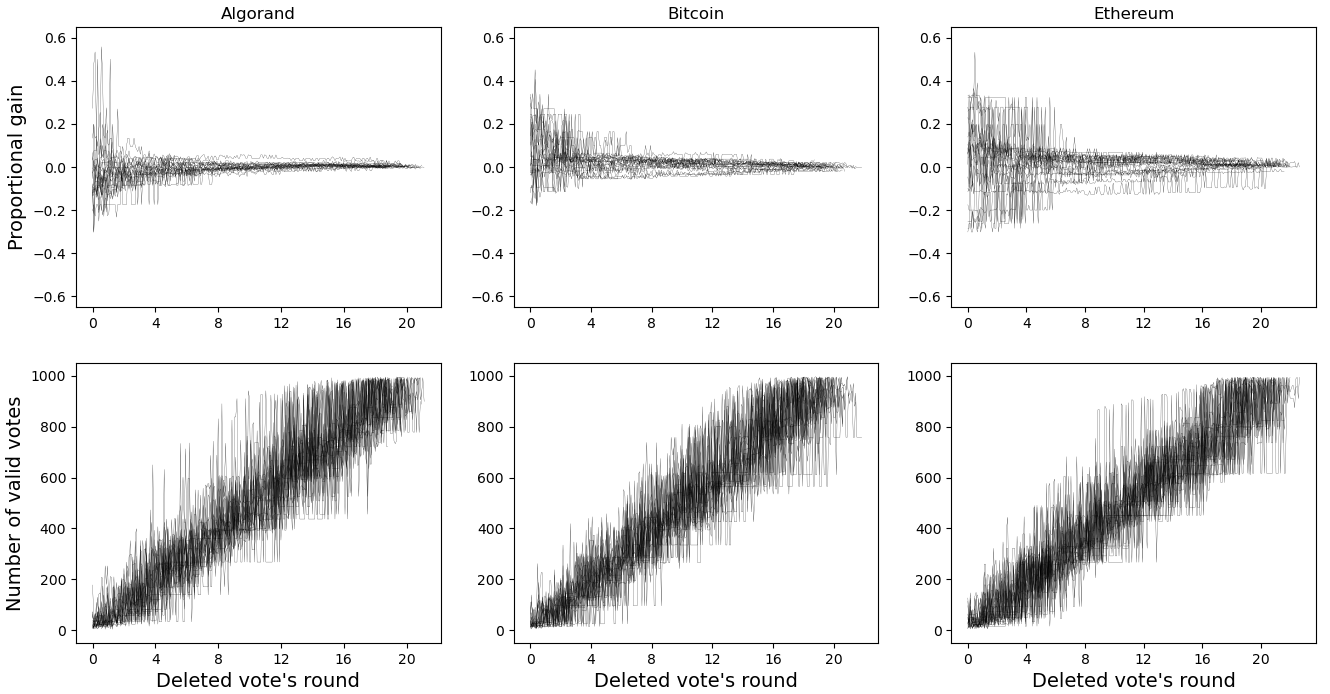
\includegraphics[width=\linewidth]{img/deleter}
	\caption{Each column denotes a different blockchain's key distribution. The top row displays the proportional gain an attacker receives by deleting the vote on the $x$-axis and the corresponding chart on the bottom row shows how many valid votes remain when the same vote is deleted. The data was gathered from 20 simulation runs for each of the three key distributions and votes are ordered on the $x$-axis by which round they were cast in.}
	\label{fig:deleter}
\end{figure}

The second strategy that we explored is called a rejecting strategy.
In the previous strategy, deleting a vote caused a chain reaction that poisoned the rest of the tangles, preserving the vote distribution.
The rejecter attempts to avoid such effects by never recording certain honest votes.
Suppose that some portion of the managers are controlled by a single, dishonest rejecter.
When a rejecter receives an honest vote submission, it will check to see if the vote's sibling is also being submitted to a manager the rejecter controls.
The rejecter will also check if it can advance its tangle without the submitted vote (because of the round requirement).
If this is the case, the manager can safely reject the vote by not recording it.
Since the vote is never recorded in the tangles, no poisoning occurs.
Then there is one less honest vote and the attacker gains a voting advantage.

\begin{figure}[h]
	\centering
	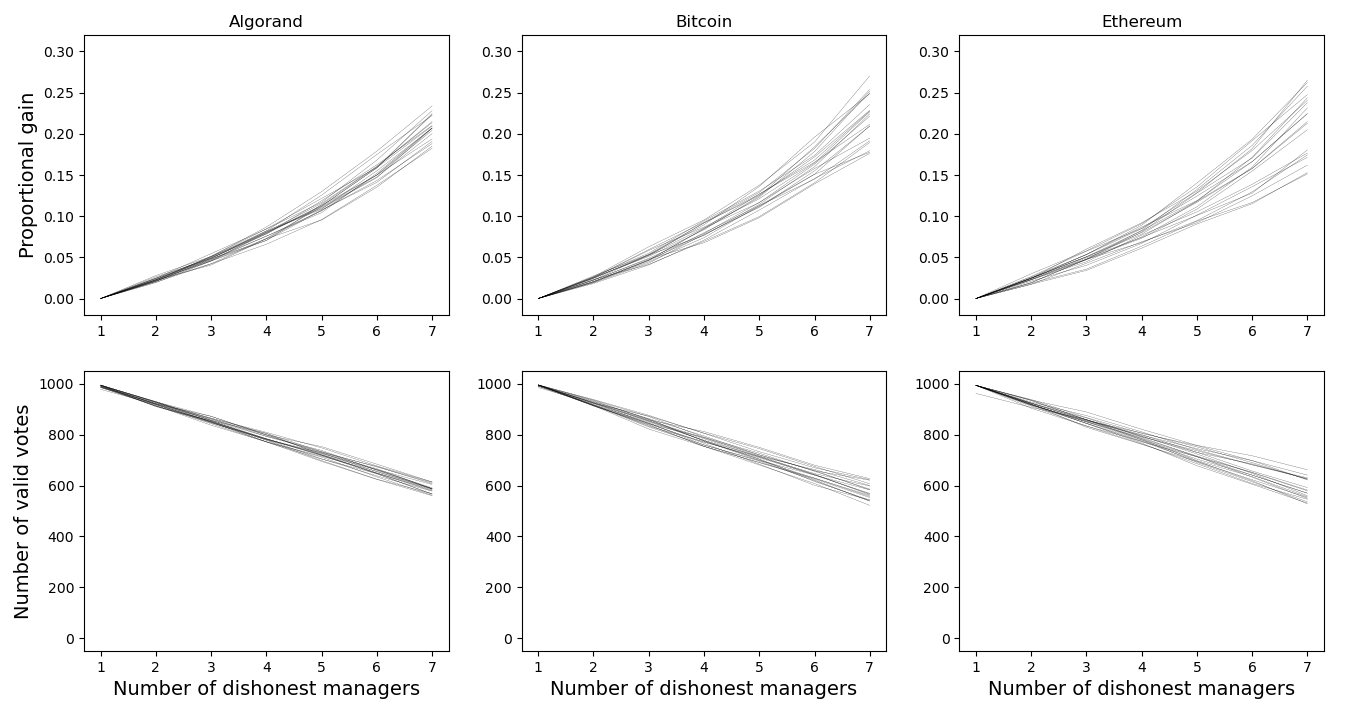
\includegraphics[width=\linewidth]{img/rejecter}
	\caption{Each column denotes a different blockchain's key distribution. The top row displays the proportional gain a rejecting attacker receives when controlling the number of dishonest managers on the $x$-axis. The corresponding chart on the bottom row shows how many valid votes remain when the same number of managers are dishonest. The data was gathered from 20 simulation runs for each of the three key distributions.}
	\label{fig:rejecter}
\end{figure}

Figure \ref{fig:rejecter} displays the effectiveness of this attack.
On the $x$-axis, we have the number of dishonest managers controlled by the same attacker.
Our simulations used 8 managers, leaving one honest manager on the right hand side of each chart.
The top row shows the proportional gain the attacker is able to collect by rejecting votes and the bottom row displays how many valid votes remain.
Algorand, Bitcoin, and Ethereum follow the same general trend: as the number of dishonest managers controlled by the rejecter increases, the gain also increases.
For each blockchain key distribution, the rejecter's gain is bounded by about 25\%.
The bottom row shows how many valid votes remain in the election.
Again, each blockchain follows the same trend.
This time, as the number of dishonest managers increases, the number of valid votes decreases.